\documentclass[12pt,a4paper]{report}
\usepackage[utf8]{inputenc}
\usepackage[top=1in,bottom=1in,left=1.5in,right=1in]{geometry}
\usepackage{graphicx}
\usepackage{tabularx}
\usepackage{subcaption}
\usepackage{multirow}
\usepackage{amsmath,amssymb,amsfonts,bbm}
\usepackage[hidelinks]{hyperref}
\usepackage{cite}
\usepackage{url} 
\usepackage{hyperref}
\usepackage{caption}
\usepackage{enumitem}
\usepackage{svg}
\usepackage{float}
\usepackage{enumitem}
\usepackage{booktabs}
\usepackage{placeins}
\usepackage[export]{adjustbox}
\usepackage{inputenc}
\usepackage{multicol}
\setlist[enumerate]{itemsep=0mm}
\DeclareUnicodeCharacter{202F}{\,} 
\newcommand\tab[1][1cm]{\hspace*{#1}} 
\setcounter{secnumdepth}{4}
\usepackage[pagestyles]{titlesec}
\titleformat
{\chapter} %command
[display]   %shape
{\Huge \bfseries} %format
{Chapter \thechapter} % chapter no format
{1ex} % separation between chapter 1 and introduction
{}
[
    \vspace{0ex}
]

\titlespacing*{\chapter}{0ex}{-2ex}{4ex}




\newcommand{\subsubsubsec}[1]{\paragraph{#1}\mbox{}\\}
\setcounter{secnumdepth}{3}

% % adjusting spacing before and after paragraphs
% \setlength{\parskip}{6pt}

% % adjusting line spacing
% \onehalfspacing

\begin{document}
      \begin{center}
		\thispagestyle{empty}
		\Large\textbf{TRIBHUVAN UNIVERSITY}\\
		\Large\textbf{INSTITUTE OF ENGINEERING }\\
		\vspace{0.2in}
		\large{\textbf{Khwopa College Of Engineering}\\}
		\normalsize{Libali, Bhaktapur\\}
		\large\textbf{Department of Computer Engineering}
		\vspace{0.2in}
		\begin{figure}[h]
		    \centering
			    
\includegraphics{img/Khwopalogo.jpg}
		\end{figure}
		
		\vspace{0.2in}
		\large{A PROPOSAL ON\\\textbf{DEEPFAKE IMAGE  DETECTION USING ResNet ARCHITECTURE}\\}
	
		\vspace{0.2in}
		\large{\textit{Submitted in partial fulfillment of the requirements for the degree\\}}
		
		\vspace{0.2in}
		\large{\textbf{BACHELOR OF COMPUTER ENGINEERING}\\}
		
		\vspace{0.2in}
		\large{Submitted by}\\
		\vspace{0.1in}
		\begin{tabular}{p{3.5in}p{2in}}
			\hspace{0.3cm}Manish Pyakurel& \hspace{1cm}KCE077BCT020\\
			\hspace{0.3cm}Rupak Neupane& \hspace{1cm}KCE077BCT028\\
			\hspace{0.3cm}Sarjyant Shrestha& \hspace{1cm}KCE077BCT033\\
			\hspace{0.3cm}Srijan Gyawali& \hspace{1cm}KCE077BCT036\\
		\end{tabular}
		\\
		\vspace{1cm}
		% \large{\textbf{Under the Supervision of}\\}
		% 	\normalsize{Er.Dinesh Gothe\\
		% 		Department Of Computer Engineering\\
		% 	}
			\vspace{0.8cm}
		\large{\textbf{Khwopa College Of Engineering}\\}
			\normalsize{Libali, Bhaktapur\\
			2023
		}
    \end{center}

  \pagenumbering{roman}
  \pagenumbering{roman}

\vspace*{1in}

\begin{center}
	\large{\textbf{CERTIFICATE OF APPROVAL}}
\end{center}
\vspace{1cm}
This is to certify that this major project work entitled \textbf{``DeepFake Image Detection"} submitted by Manish Pyakurel (KCE077BCT020), Rupak Neupane (KCE077BCT028), Sarjyant Shrestha (KCE077BCT033) and Srijan Gyawali\\(KCE077BCT036) has been examined and accepted as the partial fulfillment of the requirements for degree of Bachelor in Computer Engineering.\\
\vspace{1in}
\begin{multicols}{2}
	\begin{center}
		..........................................\\
		\textbf{Er. Himal Chand Thapa}\\
		External Examiner,\\
    Head of Department,\\
		Dept. of Computer Science and Information Technology\\
		Himalaya College of Engineering\\
		\textbf{}\\
		
	\end{center}

\columnbreak
	\begin{center}
		..........................................\\
		\textbf{Er. Subhadra Joshi}\\
		Project Supervisor,\\
    Lecturer,\\
    Dept. of Computer Engineering\\
    Khwopa College of Engineering
	\end{center}
\end{multicols}
\vspace{1in}
\begin{center}
	..........................................\\
	\textbf{Er. Dinesh Gothe}\\
	Head of Department,\\
	Department of Computer Engineering\\
	Khwopa College of Engineering
\end{center}
\pagebreak



\large
	\chapter*{Copyright}
\normalsize
\addcontentsline{toc}{section}{Copyright}
	The author has agreed that the library, Khwopa College of Engineering  may make this report freely available for inspection. Moreover, the author has agreed that permission for the extensive copying of this project report for scholarly purpose may be granted by supervisor who supervised the project work recorded here in or, in absence the Head of The Department where in the project report was done. It is understood that the recognition will be given to the author of the report and to Department of Computer Engineering, KhCE in any use of the material of this project report. Copying or publication or other use of this report for financial gain without approval of the department and author’s written permission is prohibited. Request for the permission to copy or to make any other use of material in this report in whole or in part should be addressed to: \\
	\vspace{1cm} \\
	Head of Department \\
	Department of Computer Engineering\\
	Khwopa College of Engineering\\
	Liwali,\\
	Bhaktapur, Nepal\\
\pagebreak


\large
\chapter*{Acknowledgement}
\normalsize
\addcontentsline{toc}{section}{Acknowledgement}
We extend our heartfelt gratitude to our Head of Department, Er. Dinesh Gothe, for his invaluable guidance, insightful advice, and unwavering encouragement throughout our Bachelor's program. His motivating suggestions have greatly enriched this project.\\\\
Additionally, we express our appreciation to Er. Subhadra Joshi and Er. Niranjan Bekoju for their valuable suggestions and continuous support throughout the development of this project.
\begin{table}[h]
	\begin{tabular}{@{}ll}
		Manish Pyakurel    & KCE077BCT020 \\
		Rupak Neupane      & KCE077BCT028 \\
		Sarjyant Shrestha  & KCE077BCT033 \\
		Srijan Gyawali     & KCE077BCT036 \\
	\end{tabular}
\end{table}
\pagebreak

\large
\chapter*{Abstract}
\addcontentsline{toc}{section}{Abstract}
The rise of deepfake technology, powered by advancements in deep learning, has brought a new phase to digital image manipulation. This project addresses the pressing need for a robust deepfake detection system, focusing on facial features, and employs state-of-the-art ResNet architecture. The primary goal is to develop a deep learning model capable of accurately identifying manipulated facial images. We have analysed the existing methodologies regarding deepfake technologies and detection. For this project, We used 15k Real and Fake Images from Deepfake Detection and Reconstruction Challenge as our base dataset and augmented them to a total of 50k images to train the model. We have opted to integrate CNN into the deepfake detection process, with a specific emphasis on the training and rigorous testing of the model's efficiency. We've achieved an accuracy of 93.8\% which is better than all the other proposed models in the challenge.\\\\
\textbf{Keywords}: \textit{Deepfake technology, Deep learning, Digital image manipulation, CNN}
\pagebreak

\tableofcontents
\listoffigures
\addcontentsline{toc}{section}{List of Figures}
\listoftables
\addcontentsline{toc}{section}{List of Tables}
\pagebreak

\Large
\begingroup
\let\clearpage\relax
\chapter*{List of Abbreviation}
\endgroup
\normalsize
\addcontentsline{toc}{section}{List of Abbreviations}

\begin{table}[h]
	\begin{tabular}{l l}
		\textbf{Abbreviations} & \textbf{Meaning}                                   \\
		GAN                    & Generative Adversarial Network                     \\
		CNN	                   & Convolution Neural Network                         \\
		ROC                    & Receiver Operating Characteristic                  \\
		AUC                    & Area Under The Receiver Operating Characteristics  \\
		AMTEN 								 & Adaptive Manipulation Traces Extraction Network    \\ 
		MCNet                  & Multi Level Correction Network 	                  \\
		StarGANS               & Star Generative Adversarial Networks               \\
		StyleGANS              & Style Generative Adversarial Networks              \\
		RaFT                   & Radboud Faces Database                							\\
		HFM 									 & Handcrafted Face Manipulation           						\\
		SFFM									 & Shallow-FakeFaceNet																\\
		ICIAP									 & International Conference on Image Analysis and Processing \\
	\end{tabular}
\end{table}
\pagebreak
       \chapter{Introduction}
        \pagenumbering{arabic}
        \section{Background Introduction}
        In recent years, the landscape of digital image manipulation has undergone a transformative shift with the emergence of deep fake techniques. This innovative approach, rooted in deep learning methodologies, has gained significant traction as a means of fabricating images by seamlessly replacing facial features from one individual with those of another. Coined as "deep fakes" by a Reddit user in 2017, these manipulations often leverage advanced adversarial models, such as Generative Adversarial Networks (GANs). Notably, this technology has been controversially utilized to superimpose celebrity faces onto explicit content, raising concerns related to fake pornography, misinformation, financial fraud, and hoaxes.
        Despite the ethical challenges associated with deep fakes, it is essential to acknowledge the positive applications within fields such as virtual reality, film editing, and production. The core working principles behind deep fakes involve intricate processes of merging, replacing, combining, and superimposing images. Leveraging deep learning and machine learning techniques, these manipulations give rise to convincingly altered digital images and videos, demonstrating both the potential benefits and ethical considerations associated with this rapidly advancing technology.
        \section{Problem Statement}
        In the rapidly evolving landscape of computer and automation technologies, the realm of possibilities continues to expand. Artificial Intelligence (AI) stands as a pivotal force, driving unprecedented advancements in areas such as predictive analytics, weather forecasting, automation, and the creation of sophisticated entities like deep fakes, which encompass AI-generated videos, audios, and images. While these technological strides are undeniably transformative, the misuse and exploitation of such capabilities pose significant concerns. 

        In recent times, there's been a surge in the creation of deep fakes, where the faces of celebrities or ordinary people are manipulated using just a single image and advanced deep learning algorithms. This issue is becoming more significant, as it circulates potentially harmful and illegal images of the victims to the public.

        The rise of these deceptive practices not only threatens individual privacy but also has broader implications for public trust and safety. As deep fakes become increasingly convincing, the potential for malicious use, misinformation, and damage to reputations grows. It is crucial to address this issue head-on by developing sophisticated detection mechanisms to safeguard against the harmful consequences of manipulated images. This proposal seeks to contribute to the ongoing efforts in mitigating the risks associated with deep fakes, reinforcing the integrity of visual content in the age of advanced AI technologies.
       \section{Obejctive}
            The main aim of this project is:
            \begin{itemize}
                \item To identify manipulated digital media content, particularly facial features and images.
                \item To implement cutting-edge deep learning and machine learning techniques.
            \end{itemize}
  \chapter{Literature Review}
Deepfakes, which involve the unauthorized swapping of face images, are frequently carried out without the knowledge or consent of individuals, including celebrities and politicians. Notably, historical instances, such as the facial image swapping in a photograph of Abraham Lincoln (Badale et al., 2018), underscore the longstanding nature of this challenge. Addressing these concerns, Yang, Li \& Lyu (2019) proposed a model leveraging head pose inconsistency to detect deepfakes, enabling the creation of synthetic faces for various individuals while preserving the original facial expressions.
Jagdale \& Shah (2019) introduced the NA-VSR algorithm for super resolution, involving video conversion into frames, median filtering to remove noise, and bicubic interpolation for pixel density enhancement. Additionally, Yadav \& Salmani (2019) elucidated the working principles of deep fake techniques, emphasizing the high precision value in face image swapping.
Generative Adversarial Neural Networks (GANs) play a pivotal role in deepfake generation, comprising a generator and a discriminator. The generator synthesizes fake images from a given dataset, while the discriminator evaluates the authenticity of the generated images. The inherent risks of deepfakes, including character defamation, potential harm to individuals, and the dissemination of fake news in society, highlight the importance of addressing these challenges.
Existing approaches encounter issues such as inefficiency in detecting deepfake images, high error rates, prolonged computation times, and data access inaccuracies. Our work focuses on improving the efficiency by using a different approach of using ResNet150 architecture for deepfake detection.Figure 1 presents a compilation of related works for deepfake detection (Heidari et al., 2022).

\begin{table}[ht]
  \centering
  \caption{Compilation of related work}
  \small
  \begin{tabular}{|p{2.5cm}|p{4cm}|p{2.5cm}|p{3cm}|p{3cm}|}
    \hline
    \textbf{Researcher} & \textbf{Contributions} & \textbf{Scope} & \textbf{Advantage} & \textbf{Weakness} \\
    \hline
    L. Verdoliva (2020) & Presenting an overview of contemporary manipulation techniques & Fake media & Deepfake's backstory is presented. Issues and possible solutions are explored. & There has not been any in-depth review of the articles. \\
    \hline
    Tolosana et al. (2020) & Examining face-altering techniques & Image deepfake detection & Different criteria for evaluating articles are taken into account. & It is unclear how articles are chosen for review. \\
    \hline
    Mirsky and Lee (2021) & Providing deepfake creation and detection services & Deepfake in general & Challenges and potential guidance are discussed. & It is unclear how articles are chosen for review. \\
    \hline
    Castillo Camacho and Wang (2021) & Examining DL-based image forensic methods & Image forensic & Taking into account all aspects of the criteria for image forensics. & It is unclear how articles are chosen for review. \\
    \hline
    P. Yu et al. (2021) & Focusing on deepfake video detection, its history, current research, and plans & Deepfake video & An in-depth description of future work. In-depth examination of datasets. & There is no comparison between the articles. \\
    \hline
    Rana et al. (2022) & Demonstrating several cutting-edge deepfake algorithms & DL-ML and statistical models & There is a comparison between the articles. & There is no discussion of all kinds of deepfake applications. \\
    \hline
    Ours & Providing a comprehensive review of the literature on deepfake detection techniques based on DL-based algorithms & DL-ML methods in the video, image, audio, and hybrid multimedia detection & An in-depth description of future work. In-depth examination of datasets. Challenges and potential guidance are discussed. & Papers published before 2018 are not allowed.  \\
    \hline
  \end{tabular}
\end{table}

    % L. Verdoliva (2020) & Presenting an overview of contemporary manipulation techniques & Fake media & Deepfake's backstory is presented. Issues and possible solutions are explored. There has not been any in-depth review of the articles. & \\
    % \hline
    % Tolosana et al. (2020) & Examining face-altering techniques & Image deepfake detection & Different criteria for evaluating articles are taken into account. It is unclear how articles are chosen for review. & \\
    % \hline
    % Mirsky and Lee (2021) & Providing deepfake creation and detection services & Deepfake in general & Challenges and potential guidance are discussed. It is unclear how articles are chosen for review. & \\
    % \hline
    % Castillo Camacho and Wang (2021) & Examining DL-based image forensic methods & Image forensic & Taking into account all aspects of the criteria for image forensics. It is unclear how articles are chosen for review. & \\
    % \hline
    % P. Yu et al. (2021) & Focusing on deepfake video detection, its history, current research, and plans & Deepfake video & An in-depth description of future work. In-depth examination of datasets. There is no comparison between the articles. & \\
    % \hline
    % Rana et al. (2022) & Demonstrating several cutting-edge deepfake algorithms & DL-ML and statistical models & There is a comparison between the articles. There is no discussion of all kinds of deepfake applications. & \\
    % \hline
    % Ours & Providing a comprehensive review of the literature on deepfake detection techniques based on DL-based algorithms & DL-ML methods in video, image, audio, and hybrid multimedia detection & An in-depth description of future work. In-depth examination of datasets. Challenges and potential guidance are discussed. Papers published before 2018 are not allowed. & \\
    % \hline

  \chapter{Requirement Analysis}
\section{Software Used}
    Our Deepfake Detection project requires following softwares:
    \subsection*{Python} 
    Python is our primary language for this project, chosen for its versatility and simplicity. All machine learning frameworks are imported using
    Python, leveraging its dominant position in data science and machine learning. This allows us to seamlessly integrate powerful libraries like TensorFlow and PyTorch for efficient model development.

    \subsection*{Pytorch}
    Pytorch is a an open-source machine learning framework. It provides a flexible and dynamic computational graph, which allows for easy experimentation and rapid development of deep learning models. 

    \subsection*{React}
    Through React, we can create and manage the user interface components, ensuring a smooth and interactive experience. React, being a JavaScript library, allows us to efficiently build dynamic and responsive UIs, facilitating a user-centric design approach for our project.

    \subsection*{FastAPI}
    FastAPI is a Python web framework designed for rapid API development.It serves as the primary web framework for building efficient and high-performance APIs for our project.
        
\newpage
\section{Functional Requirement}
    These are specifications that describe the fundamental capabilities and behaviors a system or product must exhibit to meet the users' needs and achieve its intended purpose. 

    \subsection{Dataset Labeler}
        Dataset labeler is the labelling system that is used to annotate the images as “Real”, or “Fake”.

    \subsection{User-Friendly Dashboard}
        A user-friendly dashboard that allows user to monitor and manage the deepfake detection process.

\section{Non-Functional Requirement}
    These are the characteristics and qualities that describe how a system should behave and perform,

    \subsection{Reliability}
        The system aims for high reliability, ensuring accurate predictions with a confidence level of 97 percent.
    \subsection{Maintainability}
        The model is designed with maintainability in mind, allowing for easy updates and further training. This ensures adaptability to evolving datasets and changing input patterns, contributing to sustained efficiency and relevance over time.
    \subsection{Portability}
        The use of standardized and widely supported libraries ensures that the model can seamlessly run on various operating systems and integrate with diverse hardware configurations.
    
\newpage
\section{Feasibility Study}
    The following points describes the feasibility of the project.

    \subsection{Economic Feasibility}
        For development of the system, all the softwares used are free of cost and hardwares were available  at reasonable cost. So,the project is economically feasible since there seems no problem with the economy for the project.

    \subsection{Technical Feasibility}
        A substantial quantity of pre-labeled datasets is readily accessible online, fulfilling a pivotal necessity for this project. Leveraging the capabilities of the Google Cloud Platform (GCP), we can meet our technical requirements efficiently, harnessing the immense processing power of the A100 80GB GPU for accelerated performance.

    \subsection{Operational Feasibility}
        The operational processes, including data labeling and model training, are well-defined and can be efficiently carried out by the project team. Additionally, the project aligns with the existing technical infrastructure and capabilities, making it operationally feasible.
      \chapter{Methodology}
       \section{Software development approach}
        Agile development is a software development approach that emphasizes incremental progress and rapid cycles. It involves releasing small increments of functionality that build upon previous versions. Thorough testing is conducted for each release to ensure software quality. Agile is often employed for time-critical applications. Although this project is not time-critical this model seems to be the most optimal and practical in our case.
        \begin{figure}[hbt!]
            \center{
                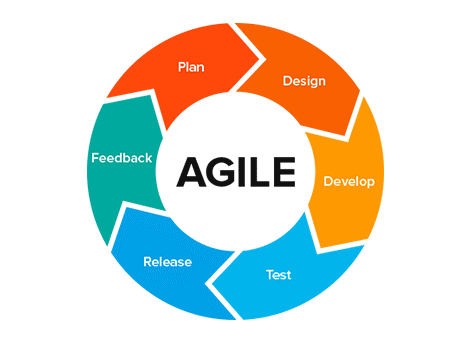
\includegraphics[width=0.75\textwidth]{./img/agile.png}
                \caption{Agile Model for Software Development}
                \subcaption*{\textit{source: \textcolor{blue}{https://mobilelive.medium.com/agile-development-a-comprehensive-guide-for-the-modern-era-d2fe9ae7b395}}}
            }
        \end{figure}

        \pagebreak

        \section{Implementation}
        \subsection{Data Collection}
        We used dataset created during a Deepfake Image Detection and Reconstruction Challenge.Two datasets of real face images were used: CelebA and FFHQ. Various Deepfake images were generated using architectures such as StarGAN, GDWCT, AttGAN, StyleGAN, and StyleGAN2. Specifically, CelebA images were manipulated using pre-trained models available on GitHub for StarGAN, GDWCT, and AttGAN. Images from StyleGAN and StyleGAN2 created through FFHQ were obtained.
        
        \begin{enumerate}
            \item CelebA\cite{7410782}: A large-scale face attributes dataset containing over 200k celebrity images with 40 labels related to facial attributes such as hair color, gender, and age. The images are in 178 x 218 JPEG format.
            
            \item FFHQ\cite{NVlabs_ffhq_dataset}: A high-quality image dataset of human faces with variations in age, ethnicity, and image background. The images are in 1024 x 1024 PNG format.
            
            \item StarGAN\cite{choi2018stargan}: Capable of performing image-to-image translations on multiple domains using a single model. CelebA images were manipulated with a pre-trained model to achieve a final resolution of 256 x 256.
            
            \item GDWCT\cite{cho2019imagetoimage}: Improves styling capability. CelebA images were manipulated with a pre-trained model to achieve a final resolution of 216 x 216.
    
            \item AttGAN\cite{8718508}: Transfers facial attributes with constraints. CelebA images were manipulated with a pre-trained model to achieve a final resolution of 256 x 256.
        
            \item StyleGAN\cite{Karras_2020_CVPR}: Transfers semantic content from a source domain to a target domain with a different style. Images were generated using FFHQ as the input dataset with a resolution of 1024 x 1024.
        
            \item StyleGAN2\cite{inproceedings}: Improves StyleGAN quality with the same task. Images were generated using FFHQ as the input dataset with a resolution of 1024 x 1024.
        \end{enumerate}
        
        \begin{figure}[hbt!]
            \centering
            \begin{minipage}{0.45\textwidth}
                    \centering
                    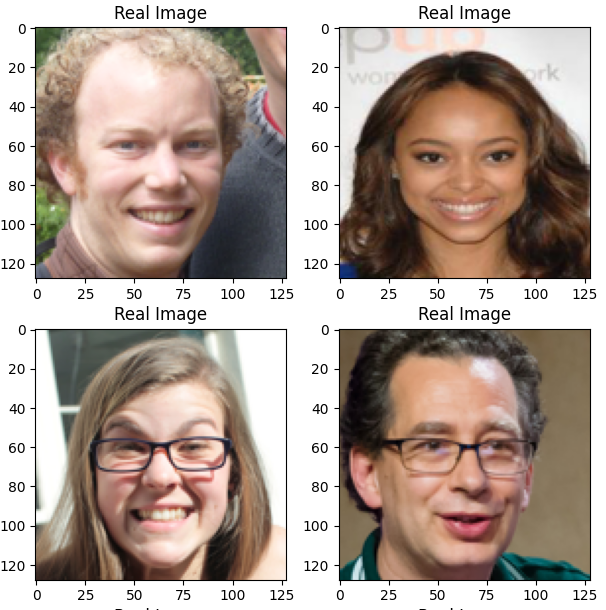
\includegraphics[width=0.95\linewidth]{./img/real sample.png}
                    \caption{Real Images}
            \end{minipage}
            \hfill
            \begin{minipage}{0.45\textwidth}
                    \centering
                    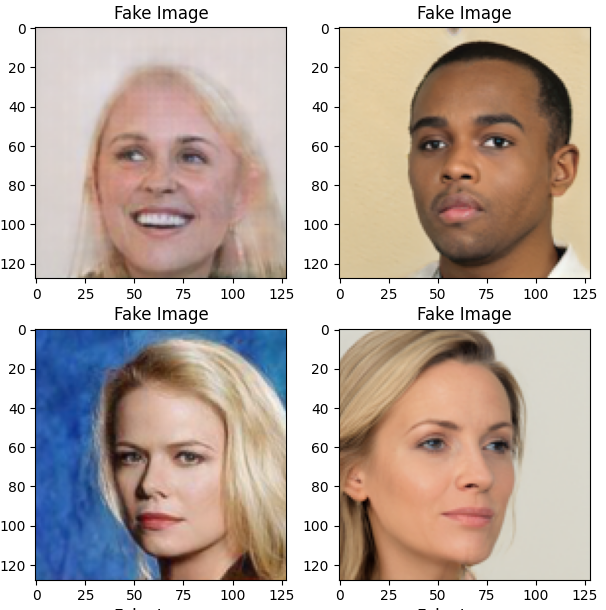
\includegraphics[width=0.95\linewidth]{./img/fake sample.png}
                    \caption{Fake Images}
            \end{minipage}
        \end{figure}

    \subsubsection{Data Augmentation}
    To balance our dataset, we augmented our images to achieve a total of 25000 images for each category. For the 5000 fake images, we applied four different transformations, resulting in 20000 augmented fake images. For the real images, we randomly selected and transformed 3750 images, generating 15000 augmented real images. \\\\
    The transformations applied were as follows:
    \begin{enumerate}
        \item Rotation: Images were rotated at an angle randomly selected from [45, 90, 135, 180, 225, 270, 315] degrees.
        \item Mirror: Images were randomly flipped horizontally, vertically, or both.
        \item Scale: Images were randomly scaled at a ratio between [0.5,2].
        \item Compression: Images were compressed using a quality factor between [50,99].
    \end{enumerate}
    After adding the augmented images to the original dataset, we ended up with a total of 25000 real and 25000 fake images.

    \subsubsection{Data Normalization}
        First, we computed the mean and standard deviation of the entire dataset, which consists of both the original dataset and the augmented dataset. The normalization process was then applied using the following formula:
        \begin{equation}
        x = \frac{x - \mu}{\sigma}
        \end{equation}
        where \(x\) represents the pixel values of each image pixel.

    \subsubsection{Data Splitting}
        We partitioned our dataset into a training set, comprising 80\% of the dataset, and a validation set, consisting of 20\% of the dataset. This division ensures that the model has an ample amount of data for learning, while also offering a subset of the data to assess the model's performance.

	\section{Data Preprocessing}
	\subsection{Data Augmentation}
		To balance our dataset, we augmented our images to achieve a total of 25000 images for each category. For the 5000 fake images, we applied four different transformations, resulting in 20000 augmented fake images. For the real images, we randomly selected and transformed 3750 images, generating 15000 augmented real images. Various transformations, such as rotation, compression, scaling, and mirroring, were implemented. A sample of each transformation is shown below:

	\begin{figure}[hbt!]
		\centering
		\begin{minipage}{0.45\textwidth}
				\centering
				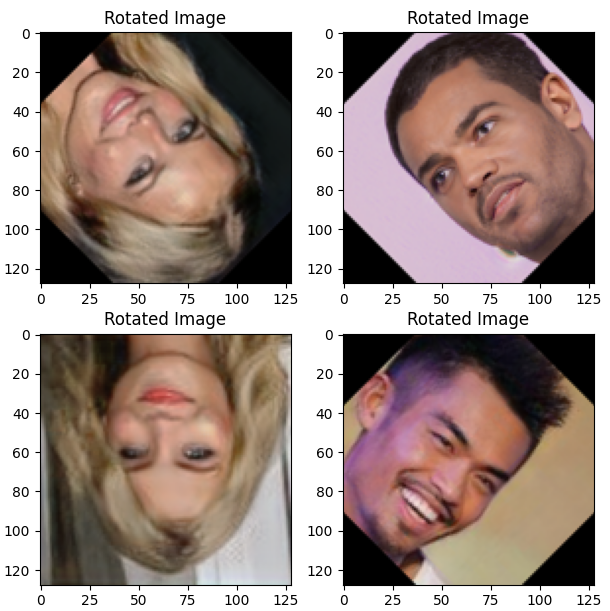
\includegraphics[width=0.95\linewidth]{./img/rotated.png}
				\caption{Rotated Images}
		\end{minipage}
		\hfill
		\begin{minipage}{0.45\textwidth}
				\centering
				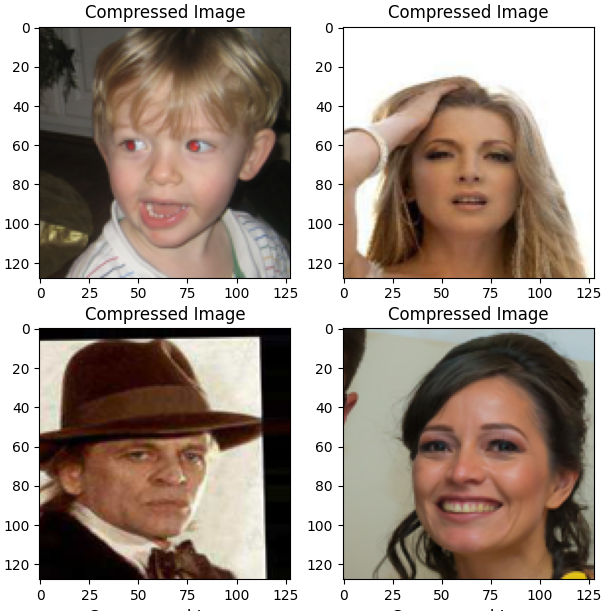
\includegraphics[width=0.95\linewidth]{./img/compressed.png}
				\caption{Compressed Images}
		\end{minipage}

		\vspace{0.5cm} % Add some vertical space between the two rows of images

		\begin{minipage}{0.45\textwidth}
				\centering
				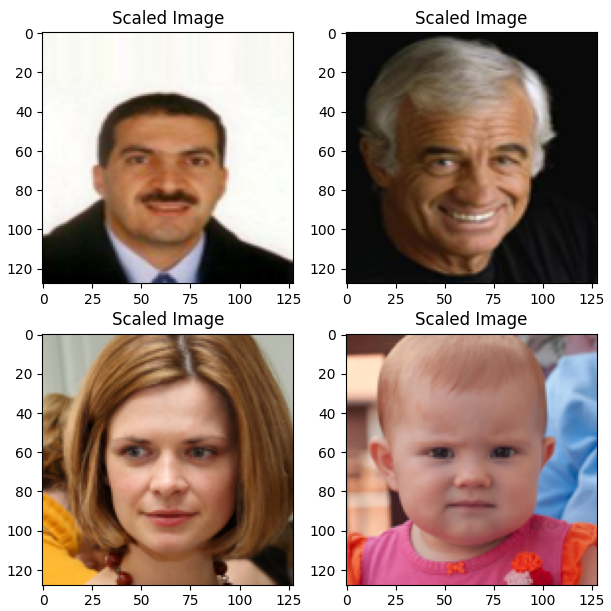
\includegraphics[width=0.95\linewidth]{./img/scaled.png}
				\caption{Scaled Image}
		\end{minipage}
		\hfill
		\begin{minipage}{0.45\textwidth}
				\centering
				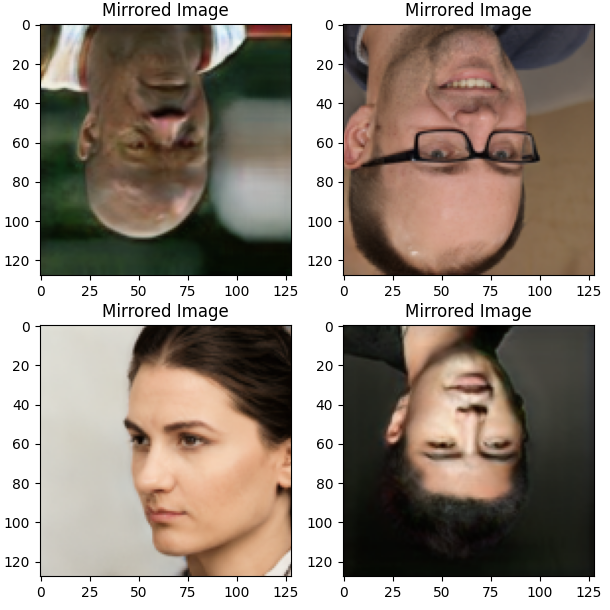
\includegraphics[width=0.95\linewidth]{./img/mirrored.png}
				\caption{Mirrored Images}
		\end{minipage}
	\end{figure}

	\subsection{Data Normalization}
	First, we computed the mean and standard deviation of the entire dataset, which consists of both the original dataset and the augmented dataset. The normalization process was then applied using the following formula:
	\begin{equation}
	x = \frac{x - \mu}{\sigma}
	\end{equation}
	where \(x\) represents the pixel values of each image pixel. \\\\
	This approach standardizes the features to have a mean of 0 and a standard deviation of 1. This standardization is crucial because certain machine learning algorithms are sensitive to the scale of the input features.

	\subsection{Data Splitting}
	We partitioned our dataset into a training set, comprising 80\% of the dataset, and a validation set, consisting of 20\% of the dataset. This division ensures that the model has an ample amount of data for learning, while also offering a subset of the data to assess the model's performance.

	\section{Setting Parameters}
	\begin{itemize}
		\item \textbf{Number of epochs : 50} \\
			The number of epochs refers to the number of times the complete training dataset is passed through the network during the training process. Each epoch consists of one forward pass (input to output) and one backward pass (error calculation and weight updates) for all the training samples.
		\item \textbf{Loss function : Cross-Entropy}\cite{mao2023crossentropy} \\
			Loss function is a method of evaluating how well your algorithm models your dataset. Cross-entropy loss measures the difference between a deep learning classification model's discovered and predicted probability distributions.

			The cross-entropy between two probability distributions, such as q from p, can be stated formally as
			
			\begin{equation}
				H(p, q) = -\sum_{x \in \mathcal{X}} p(x) \log q(x)
			\end{equation}

			Where
			\begin{itemize}
				\item H is the cross-entropy function
				\item p may be the target distribution
				\item q is the approximation of the target distribution.
			\end{itemize} 

		\item \textbf{Learning rate : 0.001} \\
			The learning rate is a hyperparameter that determines the step size at which an optimization algorithm.
		\item \textbf{Optimizer : Adam} \cite{kingma2017adam}\\
			An optimizer  is an algorithm used to update the parameters (weights and biases) of a model during training in order to minimize the loss function. 
			Adam (short for Adaptive Moment Estimation) is a popular optimization algorithm known for its robustness, efficiency, and ease of use. It often converges faster and performs better than traditional optimization algorithms.
			It adapts the learning rate for each parameter individually based on the past gradients and squared gradients making it well suited for training models.
	\end{itemize}

	\section{Model Training}
		We tested various customs models as well as pre-trained models like VGG16\_bn\cite{simonyan2015deep}, ResNet50 \cite{DBLP:journals/corr/HeZRS15}, ResNet101\cite{DBLP:journals/corr/HeZRS15}, and many more. During this process, We came to a conclusion that ResNet9 was performing much better than other models. So, We are using ResNet9 architecture for further training and implementation process.\\\\
		The model begins with an input layer configured to accept images with dimensions of 128x128 pixels and three color channels (RGB). Following this, the first convolutional layer is applied, utilizing 64 filters of size 3x3. Each filter convolves across the input image, extracting various features such as edges and textures. Batch normalization is then performed to normalize the activations of the convolutional layer, enhancing training stability. Subsequently, a rectified linear unit (ReLU) activation function is applied, introducing non-linearity to the network by replacing negative values with zeros.\\\\
		Moving forward, the second convolutional layer processes the output of the previous layer, applying 128 filters of size 3x3. Again, batch normalization and ReLU activation follow suit. Additionally, a max-pooling layer with a 2x2 window and a stride of 2 downsamples the feature maps, reducing spatial dimensions and computational complexity.\\\\
		Next, a residual block, inspired by the ResNet architecture, is introduced. This block comprises two convolutional layers, each followed by batch normalization and ReLU activation. The output of these layers is added to the output of the second convolutional layer, fostering better gradient flow during training and mitigating the vanishing gradient problem.\\\\
		Continuing, convolutional layer 3 is applied, employing 256 filters of size 3x3. Batch normalization and ReLU activation are again utilized for feature map normalization and non-linearity introduction, respectively. Another max-pooling layer further reduces spatial dimensions.\\\\
		Subsequently, convolutional layer 4 is employed, employing 512 filters of size 3x3. Similar to prior layers, batch normalization and ReLU activation are applied. Following this, another residual block, akin to ResNet architecture, is employed, aiding in feature extraction and gradient flow enhancement.\\\\
		Finally, a max-pooling layer with a 4x4 window reduces the spatial dimensions further. The resultant feature maps are then flattened into a 1D vector, which undergoes dropout regularization with a rate of 0.2, randomly deactivating 20\% of neurons during training to prevent overfitting. Lastly, a fully connected layer with two units, likely indicative of binary classification, applies a softmax activation function to generate class probabilities.
	\newpage
	\begin{figure}[hbt!]
		\center{
			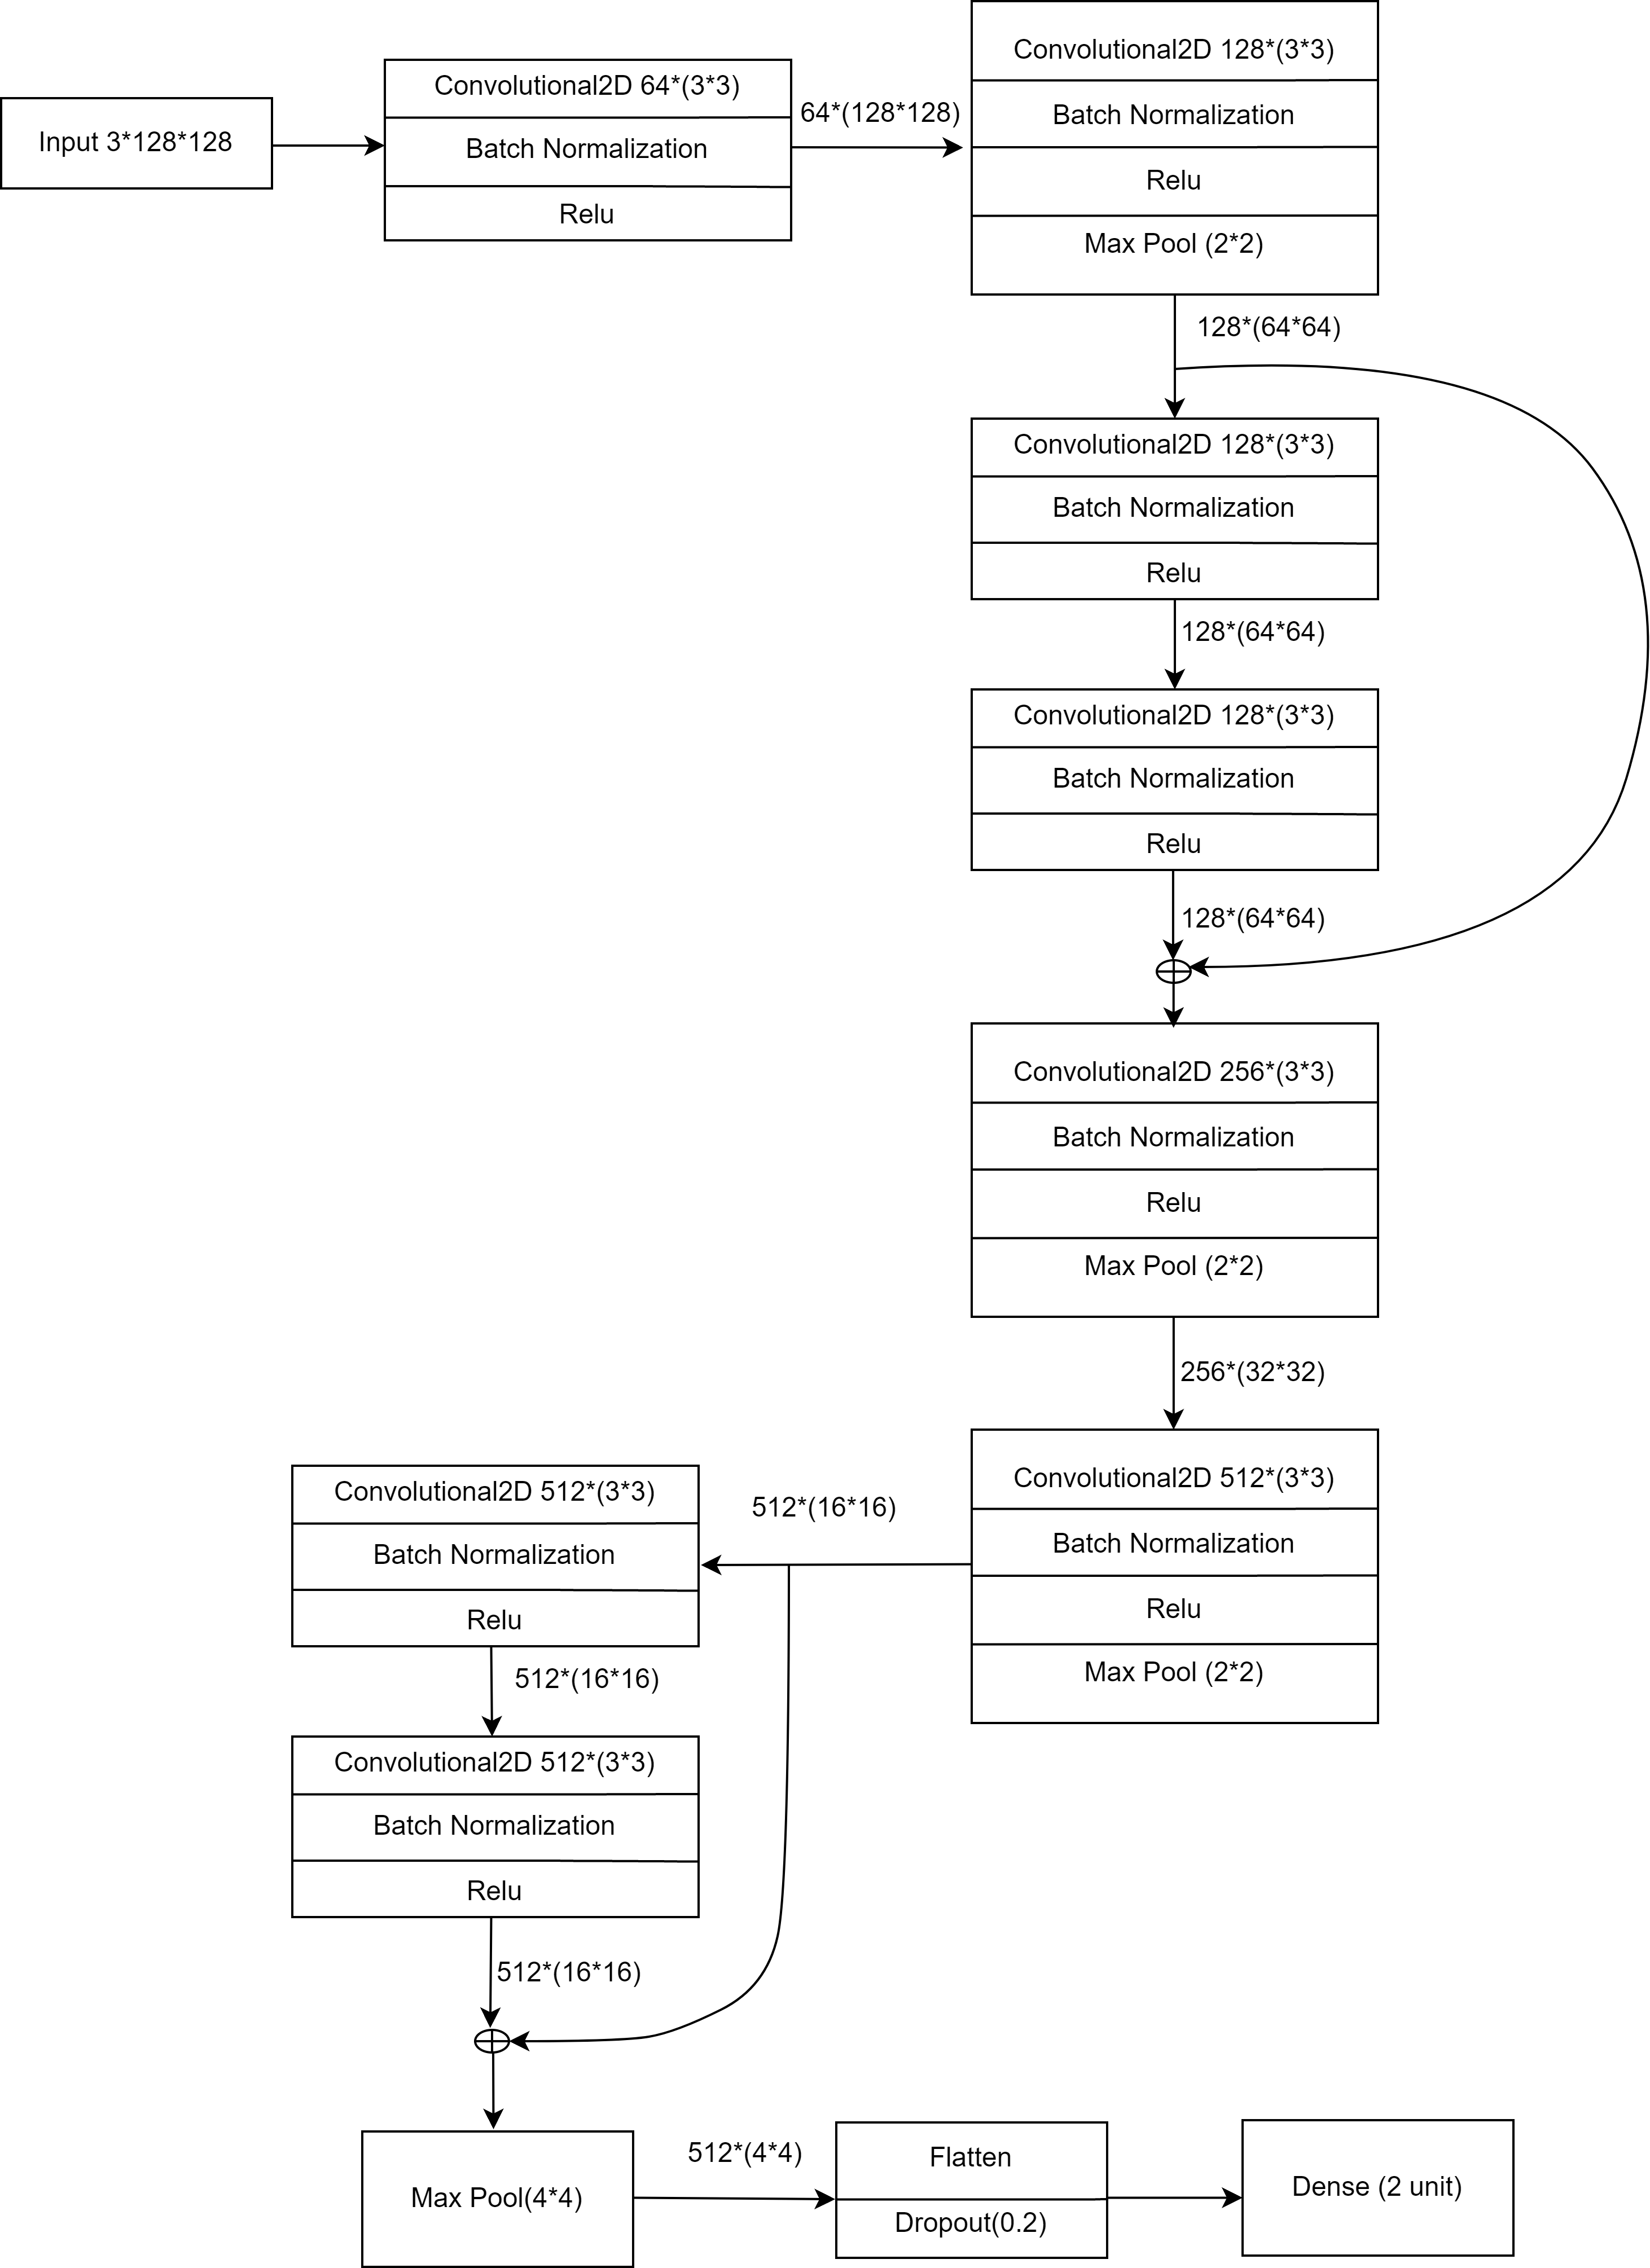
\includegraphics[width=1\textwidth]{./img/layers.png}
			\caption{Architecture of ResNet9 Model}
		}
	\end{figure}

	\clearpage
	\begin{table}
		\begin{tabular}{|l|l|l|l|}
		\hline
		\textbf{Layer} & \textbf{Layer Type} & \textbf{Output Dimension} & \textbf{No. of Parameters} \\ \hline
		1 & Input (Convolution 2-D) & (64*128*128) & 1792 \\ \hline
		2 & Batch Normalization & (64*128*128) & 256 \\      \hline
		3 & ReLU & (64*128*128) & 0 \\                       \hline
		4 & Convolution 2-D & (128*128*128) & 3584 \\        \hline
		5 & Batch Normalization & (128*128*128) & 512 \\     \hline
		6 & ReLU & (128*128*128) & 0 \\                      \hline
		7 & MaxPooling & (128*64*64) & 0 \\                  \hline
		8 & Convolution 2-D & (128*64*64) & 3584 \\          \hline
		9 & Batch Normalization & (128*64*64) & 512 \\       \hline
		10 & ReLU & (128*64*64) & 0 \\                       \hline
		11 & Convolution 2-D & (128*64*64) & 3584 \\         \hline
		12 & Batch Normalization & (128*64*64) & 512 \\      \hline
		13 & ReLU & (128*64*64) & 0 \\                       \hline
		14 & Convolution 2-D & (256*64*64) & 7168 \\         \hline
		15 & Batch Normalization & (256*64*64) & 1024 \\     \hline
		16 & ReLU & (128*64*64) & 0 \\                       \hline
		17 & MaxPooling & (256*32*32) & 0 \\                 \hline
		18 & Convolution 2-D & (512*32*32) & 14336 \\        \hline
		19 & Batch Normalization & (512*32*32) & 2048 \\     \hline
		20 & ReLU & (512*32*32) & 0 \\                       \hline
		21 & MaxPooling & (512*16*16) & 0 \\                 \hline
		22 & Convolution 2-D & (512*16*16) & 14336 \\        \hline
		23 & Batch Normalization & (512*16*16) & 2048 \\     \hline
		24 & ReLU & (512*16*16) & 0 \\                       \hline
		25 & Convolution 2-D & (512*16*16) & 14336 \\        \hline
		26 & Batch Normalization & (512*16*16) & 2048 \\     \hline
		27 & ReLU & (512*16*16) & 0 \\                       \hline
		28 & MaxPooling & (512*4*4) & 0 \\                   \hline
		29 & Flatten & 8192 & 0 \\                           \hline
		30 & DropOut & 8192 & 0 \\                           \hline
		31 & Dense & 2 & 16386 \\\hline
		\end{tabular}
	\end{table}

	\begin{table}[ht]
		\begin{tabularx}{1.03\textwidth}{|X|X|}
			\hline
			Total Parameters & 16386 \\ \hline
			Trainable Parameters & 16386 \\  \hline
			Non-Trainable Parameters & 0 \\ \hline
			\end{tabularx}
			\caption{Output Dimensions and Parameter for Each Layer}
		\end{table}
        
        
        \subsection{CNN}
            A Convolutional Neural Network (CNN) \cite{oshea2015introduction} is a Deep Learning algorithm
            that can take in an input image, assign importance (learnable weights and biases) to various aspects/objects in the image, and be able to differentiate one from the other. The pre-processing required in a CNN is much lower as compared to other classification algorithms. While in primitive methods filters are hand-engineered, with enough training, CNNs have the ability to learn these filters characteristics.The architecture of a CNN is analogous to that of the connectivity pattern of Neurons in the Human Brain and was inspired by the organization of the Visual Cortex. Individual neurons respond to stimuli only in a restricted region of the visual field known as the Receptive Field. A collection of such fields overlap to cover the entire visual area.A CNN typically has three layers: a convolutional layer, a pooling layer, and a fully connected layer.

        \begin{figure}[hbt!]
                \center{
                    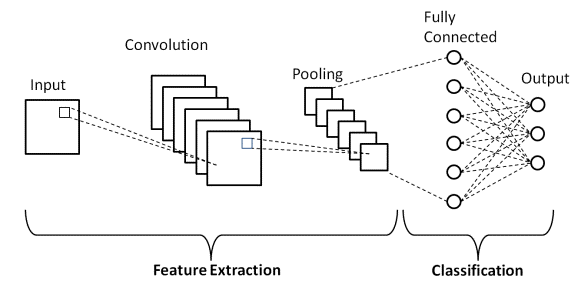
\includegraphics[width=0.85\textwidth]{./img/CNN.png}
                }
                \caption{Convolutional Neural Networks} \cite{E1ICAW_2018_v16n3_173}
        \end{figure}

        \newpage
        \subsection{ResNet}
            ResNet\cite{DBLP:journals/corr/HeZRS15} architecture introduced the concept called Residual Blocks. In this network, we use a technique called skip connections. The skip connection connects activations of a  layer to further layers by skipping some layers in between. This forms a residual block. Resnets are made by stacking these residual blocks together. The approach behind this network is instead of layers learning the underlying mapping, we allow the network to fit the residual mapping. So, instead of say H(x), initial mapping, let the network fit,
            \begin{equation}
                F(x) := H(x) - x
            \end{equation}
            which gives
            \begin{equation}
                H(x) := F(x) + x
            \end{equation}
            \begin{figure}[hbt!]
                \center{
                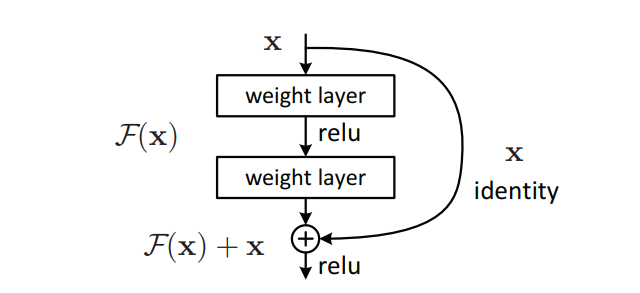
\includegraphics[width=1\textwidth]{./img/ResNet.PNG}
                }
                \caption{ResNet} \cite{enwiki:1205293224}
            \end{figure}

        
        % \subsection{GanttChart}
        %     \begin{figure}[hbt!]
        %         \center{
        %             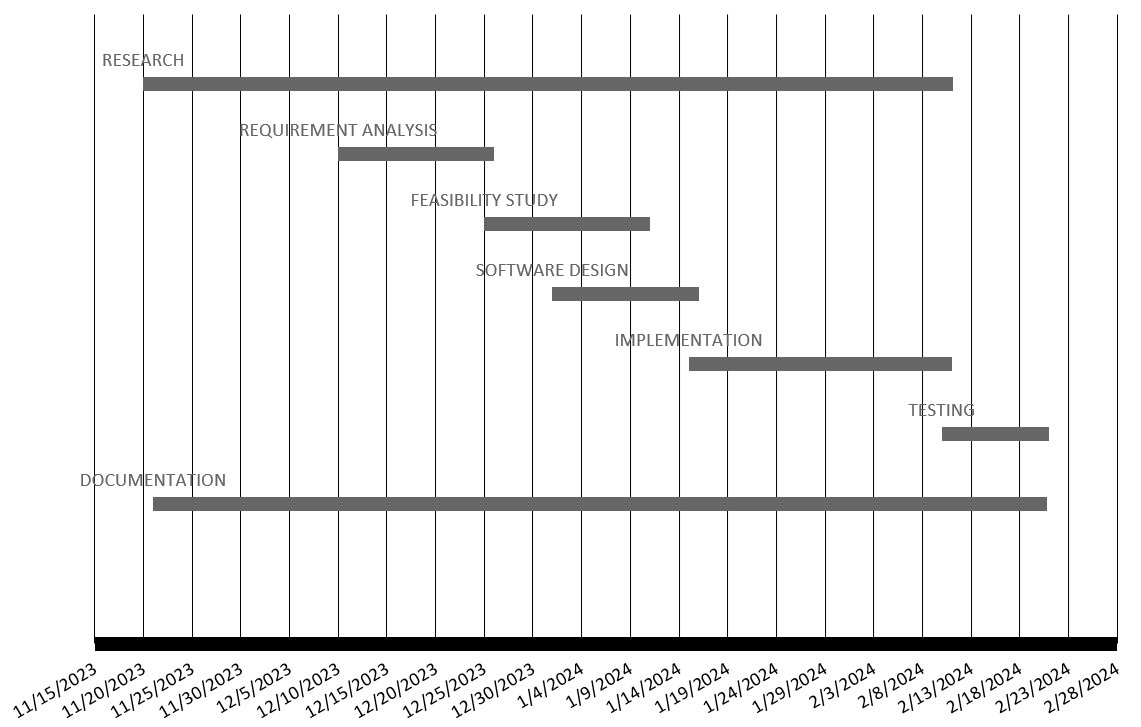
\includegraphics[width=0.1\textwidth]{./img/GANT_CHART.jpg}
        %         }
        %         \caption{Gantt chart}
        %     \end{figure}

  \chapter{Work Completed}
	\section{Data Accumulation}
		We used dataset created during a Deepfake Image Detection and Reconstruction
		Challenge. Two datasets of real face images were used: CelebA and FFHQ. Various
		Deepfake images were generated using architectures such as StarGAN, GDWCT,
		AttGAN, StyleGAN, and StyleGAN2. Specifically, CelebA images were manipulated
		using pre-trained models available on GitHub for StarGAN, GDWCT, and AttGAN.
		Images from StyleGAN and StyleGAN2 created through FFHQ were obtained. A sample of real and fake images are shown below:

	\begin{figure}[hbt!]
		\centering
		\begin{minipage}{0.45\textwidth}
				\centering
				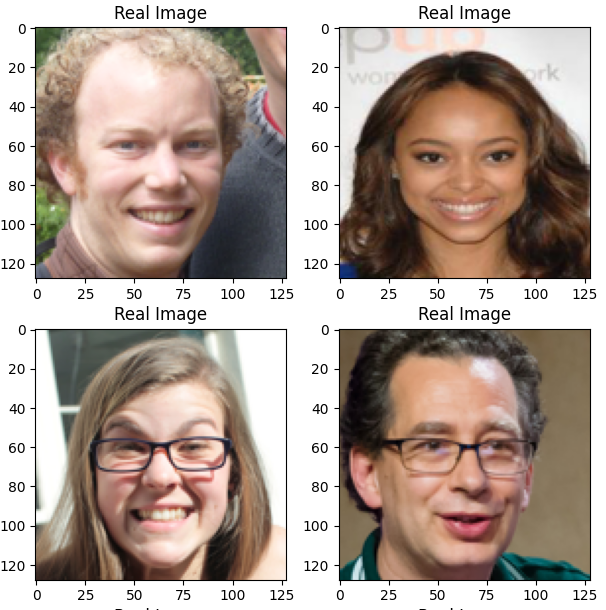
\includegraphics[width=0.95\linewidth]{./img/real sample.png}
				\caption{Real Images}
		\end{minipage}
		\hfill
		\begin{minipage}{0.45\textwidth}
				\centering
				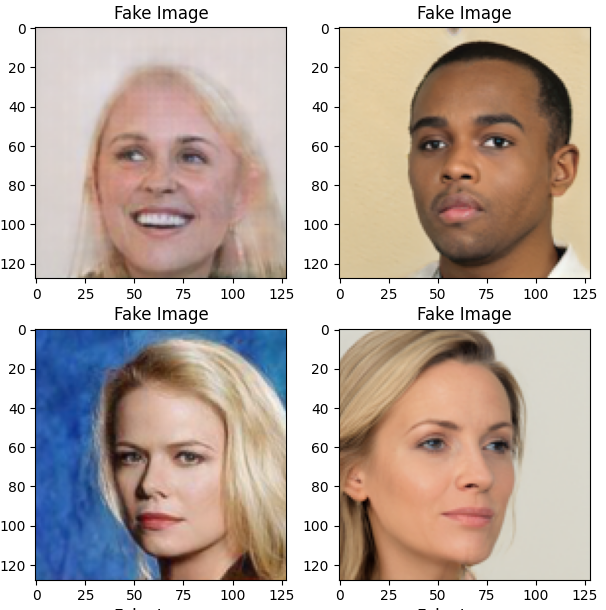
\includegraphics[width=0.95\linewidth]{./img/fake sample.png}
				\caption{Fake Images}
		\end{minipage}
	\end{figure}

	\section{Data Preprocessing}
	\subsection{Data Augmentation}
		To balance our dataset, we augmented our images to achieve a total of 25000 images for each category. For the 5000 fake images, we applied four different transformations, resulting in 20000 augmented fake images. For the real images, we randomly selected and transformed 3750 images, generating 15000 augmented real images. Various transformations, such as rotation, compression, scaling, and mirroring, were implemented. A sample of each transformation is shown below:

	\begin{figure}[hbt!]
		\centering
		\begin{minipage}{0.45\textwidth}
				\centering
				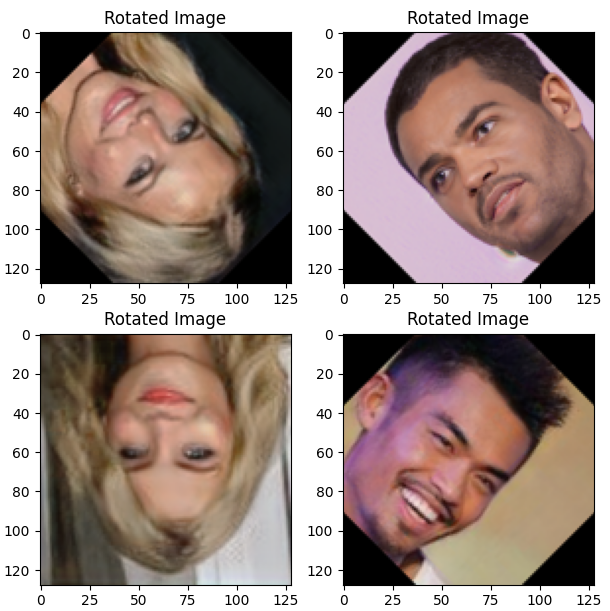
\includegraphics[width=0.95\linewidth]{./img/rotated.png}
				\caption{Rotated Images}
		\end{minipage}
		\hfill
		\begin{minipage}{0.45\textwidth}
				\centering
				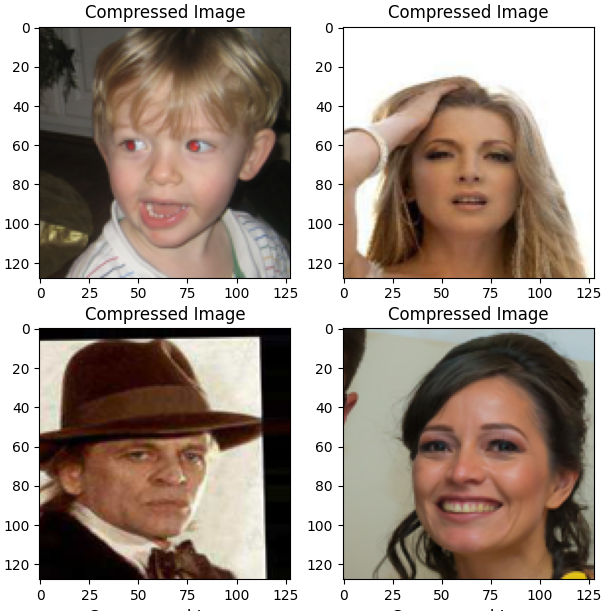
\includegraphics[width=0.95\linewidth]{./img/compressed.png}
				\caption{Compressed Images}
		\end{minipage}

		\vspace{0.5cm} % Add some vertical space between the two rows of images

		\begin{minipage}{0.45\textwidth}
				\centering
				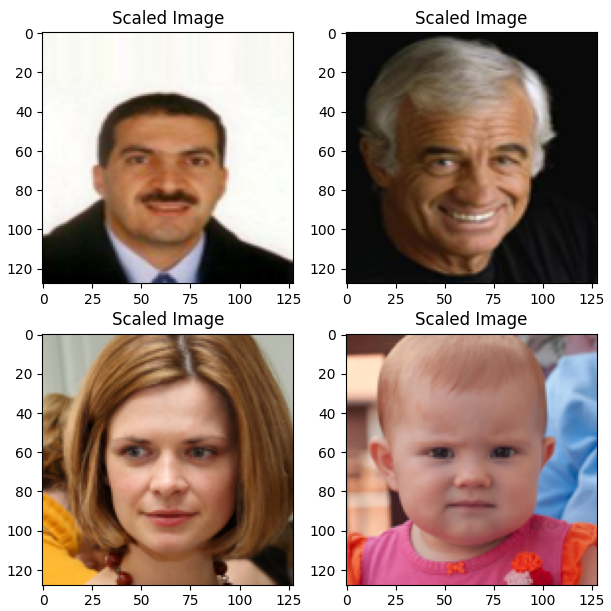
\includegraphics[width=0.95\linewidth]{./img/scaled.png}
				\caption{Scaled Image}
		\end{minipage}
		\hfill
		\begin{minipage}{0.45\textwidth}
				\centering
				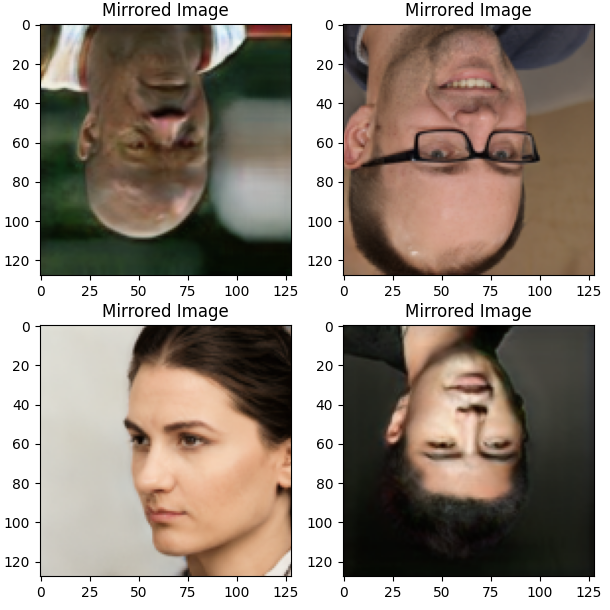
\includegraphics[width=0.95\linewidth]{./img/mirrored.png}
				\caption{Mirrored Images}
		\end{minipage}
	\end{figure}

	\subsection{Data Normalization}
	First, we computed the mean and standard deviation of the entire dataset, which consists of both the original dataset and the augmented dataset. The normalization process was then applied using the following formula:
	\begin{equation}
	x = \frac{x - \mu}{\sigma}
	\end{equation}
	where \(x\) represents the pixel values of each image pixel.
	
	This approach standardizes the features to have a mean of 0 and a standard deviation of 1. This standardization is crucial because certain machine learning algorithms are sensitive to the scale of the input features.

	\subsection{Data Splitting}
	We partitioned our dataset into a training set, comprising 80\% of the dataset, and a validation set, consisting of 20\% of the dataset. This division ensures that the model has an ample amount of data for learning, while also offering a subset of the data to assess the model's performance.

	\section{Setting Parameters}
	\begin{itemize}
		\item \textbf{Number of epochs : 50} \\
			The number of epochs refers to the number of times the complete training dataset is passed through the network during the training process. Each epoch consists of one forward pass (input to output) and one backward pass (error calculation and weight updates) for all the training samples.
		\item \textbf{Loss function : Cross-Entropy} \\
			Loss function is a method of evaluating how well your algorithm models your dataset. Cross-entropy loss measures the difference between a deep learning classification model's discovered and predicted probability distributions.

			The cross-entropy between two probability distributions, such as q from p, can be stated formally as
			
			\begin{equation}
				H(p, q) = -\sum_{x \in \mathcal{X}} p(x) \log q(x)
			\end{equation}

			Where
			\begin{itemize}
				\item H is the cross-entropy function
				\item p may be the target distribution
				\item q is the approximation of the target distribution.
			\end{itemize} 

		\item \textbf{Learning rate : 0.001} \\
			The learning rate is a hyperparameter that determines the step size at which an optimization algorithm.
		\item \textbf{Optimizer : Adam} \\
			An optimizer  is an algorithm used to update the parameters (weights and biases) of a model during training in order to minimize the loss function. 
			Adam (short for Adaptive Moment Estimation) is a popular optimization algorithm known for its robustness, efficiency, and ease of use. It often converges faster and performs better than traditional optimization algorithms.
			It adapts the learning rate for each parameter individually based on the past gradients and squared gradients making it well suited for training models.
	\end{itemize}

	\section{Model Training}
		We tested various customs models as well as pre-trained models like VGG16\_bn, ResNet50, ResNet101, and many more. During this process, We came to a conclusion that ResNet9 was performing much better than other models. So, We are using ResNet9 architecture for further training and implementation process.
		
		The model begins with an input layer configured to accept images with dimensions of 128x128 pixels and three color channels (RGB). Following this, the first convolutional layer is applied, utilizing 64 filters of size 3x3. Each filter convolves across the input image, extracting various features such as edges and textures. Batch normalization is then performed to normalize the activations of the convolutional layer, enhancing training stability. Subsequently, a rectified linear unit (ReLU) activation function is applied, introducing non-linearity to the network by replacing negative values with zeros.

		Moving forward, the second convolutional layer processes the output of the previous layer, applying 128 filters of size 3x3. Again, batch normalization and ReLU activation follow suit. Additionally, a max-pooling layer with a 2x2 window and a stride of 2 downsamples the feature maps, reducing spatial dimensions and computational complexity.

		Next, a residual block, inspired by the ResNet architecture, is introduced. This block comprises two convolutional layers, each followed by batch normalization and ReLU activation. The output of these layers is added to the output of the second convolutional layer, fostering better gradient flow during training and mitigating the vanishing gradient problem.

		Continuing, convolutional layer 3 is applied, employing 256 filters of size 3x3. Batch normalization and ReLU activation are again utilized for feature map normalization and non-linearity introduction, respectively. Another max-pooling layer further reduces spatial dimensions.

		Subsequently, convolutional layer 4 is employed, employing 512 filters of size 3x3. Similar to prior layers, batch normalization and ReLU activation are applied. Following this, another residual block, akin to ResNet architecture, is employed, aiding in feature extraction and gradient flow enhancement.

		Finally, a max-pooling layer with a 4x4 window reduces the spatial dimensions further. The resultant feature maps are then flattened into a 1D vector, which undergoes dropout regularization with a rate of 0.2, randomly deactivating 20\% of neurons during training to prevent overfitting. Lastly, a fully connected layer with two units, likely indicative of binary classification, applies a softmax activation function to generate class probabilities.
	\newpage
	\begin{figure}[hbt!]
		\center{
			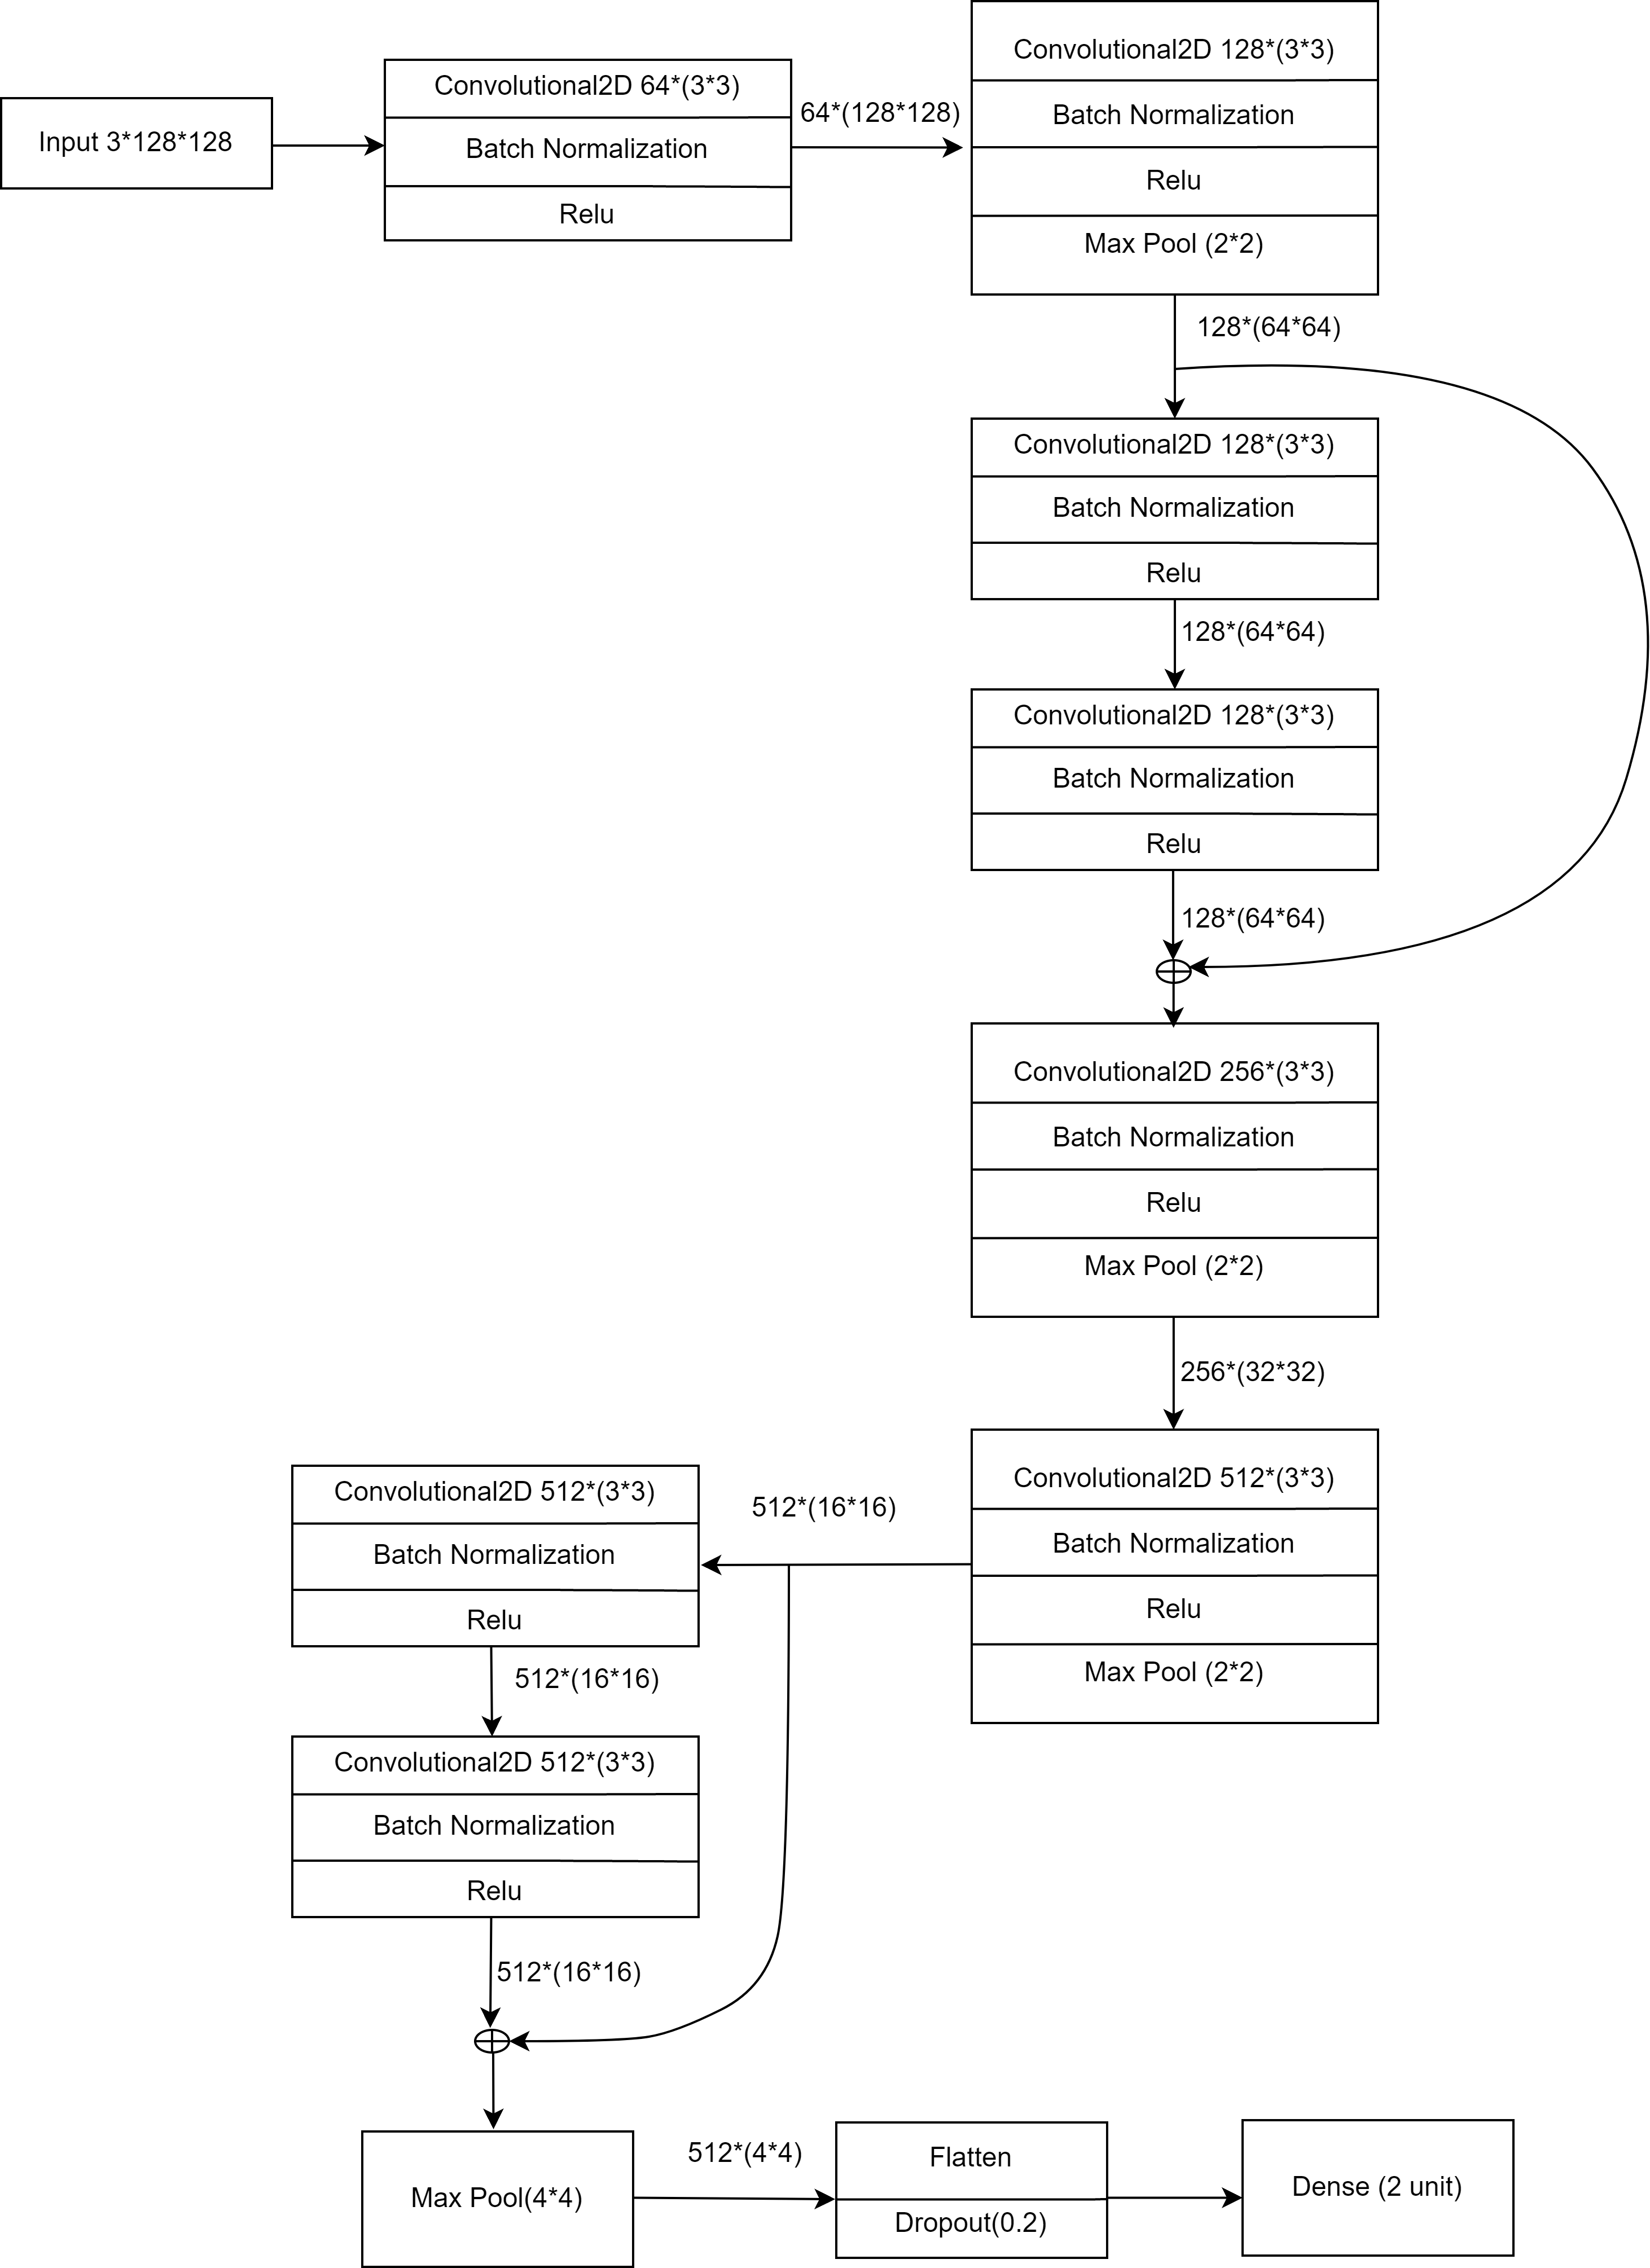
\includegraphics[width=0.68\textheight]{./img/layers.png}
			\caption{Architecture of ResNet9 Model}
		}
	\end{figure}

	\section{Model Evaluation}
	\begin{figure}[hbt!]
		\center{
			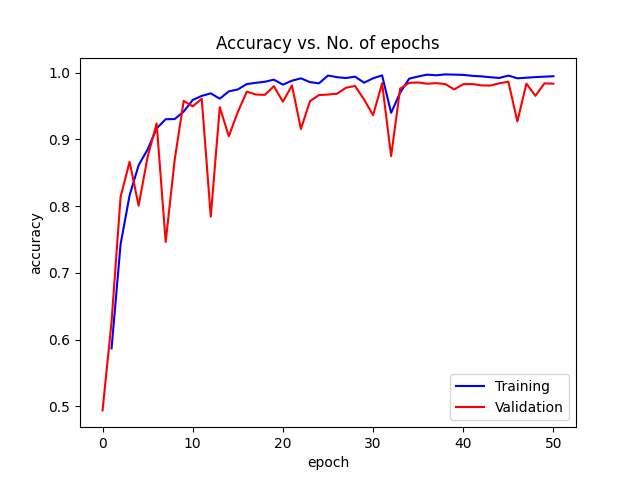
\includegraphics[width=0.8\textwidth]{./img/resnet9accuracy.png}
			\caption{Accuracy vs. No. of epochs }
		}
	\end{figure}
	\begin{figure}[hbt!]
		\center{
			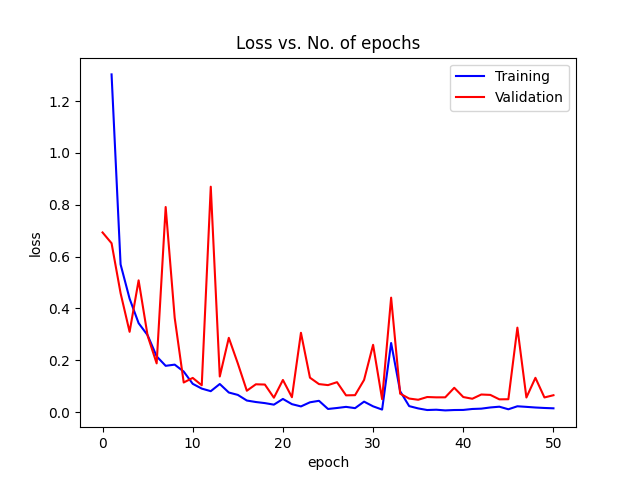
\includegraphics[width=0.8\textwidth]{./img/resnet9losses.png}
			\caption{Loss vs. No. of epochs}
		}
	\end{figure}

	\subsection*{Testing Results}
	We used the test dataset given on the DeepFake Detection Challenge\cite{jimaging8100263} to test our models performance.
	Testing dataset consist of 5000 fake images and 2000 real images.
	\vspace{1pt}
	\begin{figure}[hbt!]
		\center{
			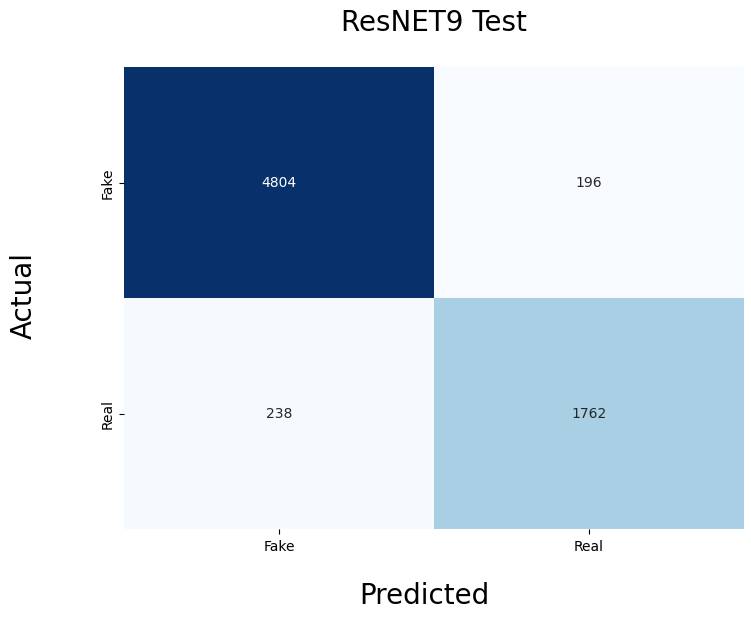
\includegraphics[width=1\textwidth]{./img/confusion_matrix.png}
			\caption{Confusion Matrix}
		}
	\end{figure}

	% \newpage
	\begin{enumerate}
		\item Accuracy
		\begin{equation}
				\text{Accuracy} = \frac{\text{TP} + \text{TN}}{\text{TP} + \text{TN} + \text{FP} + \text{FN}}
		\end{equation}
		\item Precision
		\begin{equation}
			% \begin{flalign}
				\text{Precision} = \frac{\text{TP}}{\text{TP} + \text{FP}}
			% \end{flalign}
		\end{equation}
		\item Recall
		\begin{equation}
			\text{Recall} = \frac{\text{TP}}{\text{TP} + \text{FN}}
		\end{equation}
		\item F1 Score
		\begin{equation}
			\text{F1 Score} = 2 \times \frac{\text{Precision} \times \text{Recall}}{\text{Precision} + \text{Recall}}
		\end{equation}

		where
		TP = True Positive,
		TN = True Negative,
		FP = False Positive,
		FN = False Negative
		\item Reciever Operating Characteristic (ROC) Curve
			\begin{figure}[hbt!]
				\center{
					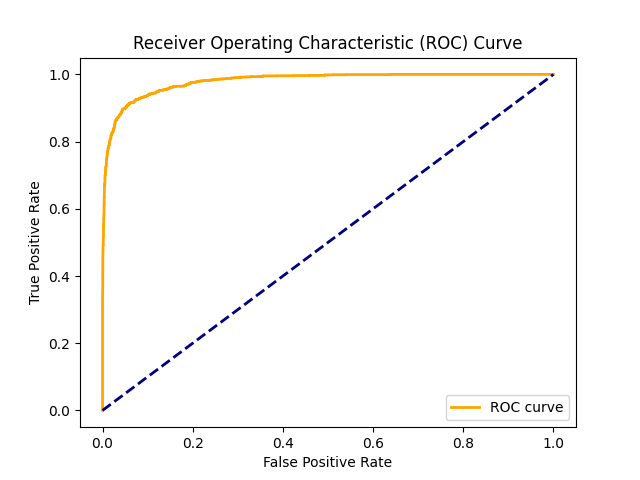
\includegraphics[width=1\textwidth]{./img/ROC.png}
					\caption{Reciever Operating Characteristic (ROC) Curve}
				}
			\end{figure}

			\textbf{Area Under ROC Curve = 0.9796}

\begin{table}[h!]
		\centering
		\begin{tabular}{lccccc}
		\multicolumn{6}{c}{\textbf{}} \\ 
		\multicolumn{6}{c}{\textbf{}} \\ 
		\textbf{} & \textbf{Accuracy} & \textbf{Precision} & \textbf{Recall} & \textbf{F1-score} & \textbf{Support} \\
		\textbf{Fake}  & 96.08\% & 0.952 & 0.960 & 0.955 & 5000 \\
		\textbf{Real} & 88.10\%  & 0.899 & 0.881 & 0.889 & 2000 \\
		\textbf{Macro Avg} & 92.09\% & 0.925 & 0.920 & 0.922 & 7000 \\
		\textbf{Weighted Avg} & 93.80\% & 0.936 & 0.938 & 0.937 &7000 \\ 
		\multicolumn{6}{c}{\textbf{}} \\
		\multicolumn{6}{c}{\textbf{}} \\
		\end{tabular}
		\caption{Performance Table}
		\end{table}
\end{enumerate}

\newpage
\section{User Interface}

\begin{figure}[hbt!]
	\center{
		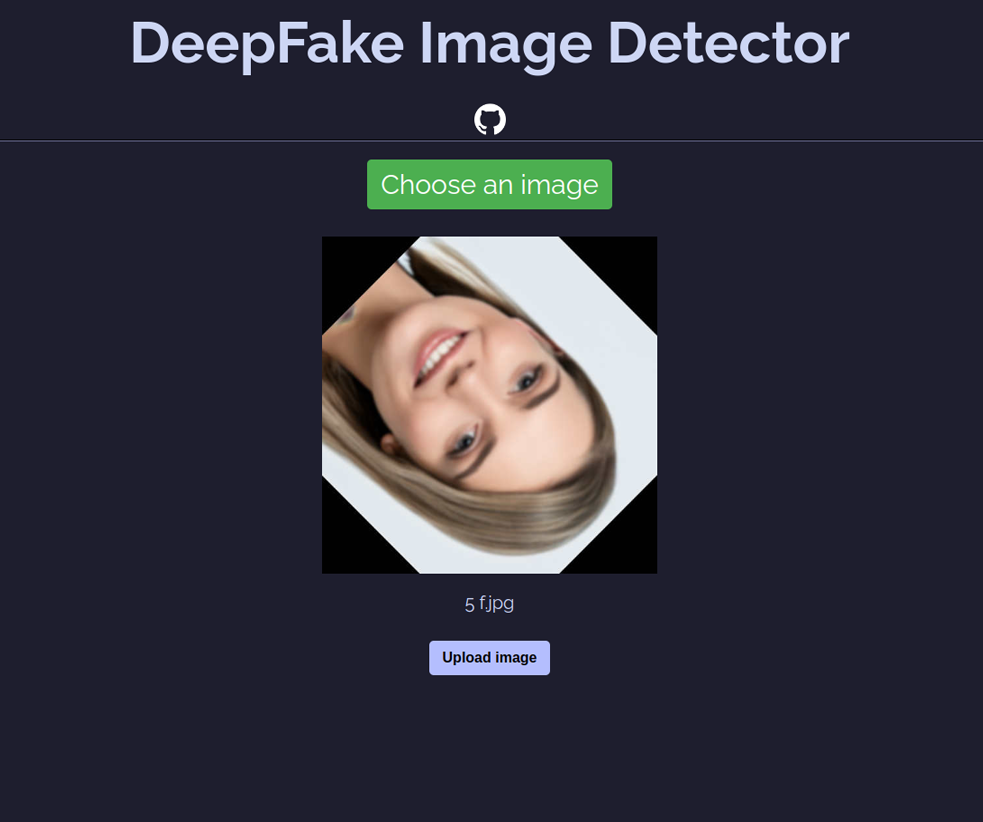
\includegraphics[width=0.66\textwidth]{./img/UI1.png}
		\caption{Demonstration of model detecting real image}
	}
\end{figure}
\begin{figure}[hbt!]
	\center{
		
\includegraphics[width=0.66\textwidth]{./img/UI2.jpg}
		\caption{Demonstration of model detecting fake image}
	}
\end{figure}
  	\chapter{Expected Outcomes}
    	The labelling system work properly. Sentences from the database were properly displayed in the web application. Labeler successfully labelled about 5,680 data points which was stored in 512KB chunks of files. The system for labelling Nepali sentiment sentences has been completed. The input data from the file was successfully retrieved, then preprocessed and sent to the model for training.
    	\vspace{0.2in}
    	Various models for sentiment classification was trained and the results of the training are shown in the table below:
    	
\begin{center}
    \begin{tabular}{|p{1cm}|p{3cm}|p{4cm}|p{4cm}|p{2cm}| }
        \hline
        S.N. & Model & Training Accuracy & Testing Accuracy & Epochs\\
        \hline
        1. & LSTM RNN Model & 80\% & 82\% & 3\\
        \hline
        2. & Attention Based LSTM RNN & 88\% & 80\% & 5 \\
        \hline
        3. & POS integrated LSTM RNN & 86\% & 74.5\% & 4 \\
        \hline
        4. & Attention based POS integrated LSTM RNN  & 89\% & 75\% & 4 \\
        \hline
    \end{tabular}
    \begin{figure}[h]
	    \centering
		    \includegraphics[width=0.75\textwidth]{./img/7.1.jpg}
		    \caption{Confusion matrix for LSTM RNN Model}
	\end{figure}
\end{center}	
	The best model was found to be LSTM RNN Model with testing accuracy 82\%, recall 87\%, precision of 76\%. Other models performed worse than this model was due to added complexity for low datapoints. After building the basic LSTM model we tried to 
	increase its accuracy by changing various variables such as changing word embedding, adding POS feature to the basic model but, due to low number of datapoints for added complexity in the model, they started overfitting. To solve the problem of overfitting of the model we tried different measures such as dropout, regularization and increasing data. But increasing data was not an option for us due to limited time.\\\\
	increase its accuracy by changing various variables such as changing word embedding, adding POS feature to the basic model but, due to low number of datapoints for added complexity in the model, they started overfitting. To solve the problem of overfitting of the model we tried different measures such as dropout, regularization and increasing data. But increasing data was not an option for us due to limited time.
  \newpage
  \bibliographystyle{unsrt}
  \bibliography{references}
\end{document}